\section{Processos de fabricação}

Até o ponto de controle 2 toda a estrutura interna e parte da externa foram fabricadas. A seguir tem-se os materiais utilizados para cada um e como se deu o processo de fabricação.

\section{Estrutura interna}

Materiais:
\begin{itemize}
	\item	Barras de metalon
	\item	Chapas de alumínio
	\item	Corrediças telescópicas
\end{itemize}

Fabricação:
\begin{itemize}
	\item	As barras de metalon foram soldadas para dar forma ao chassi.
	\item	Uma chapa de alumínio foi cortada na cortadora de chapas e em seguida foi rebitada no chassi para fazer o fundo da estrutura.
	\item	As corrediças telescópicas foram presas no chassi com parafusos, e tais furos foram feitos com a fresadora.
	\item	Uma outra chapa de alumínio foi cortada na cortadora de chapas e em seguida dobrada na dobradeira de chapas para fazer a gaveta onde comportará as mudas.
\end{itemize}

As figuras de 44 a 46 apresentam os resultados da estrutura interna.

\begin{figure}[H]
	\centering
	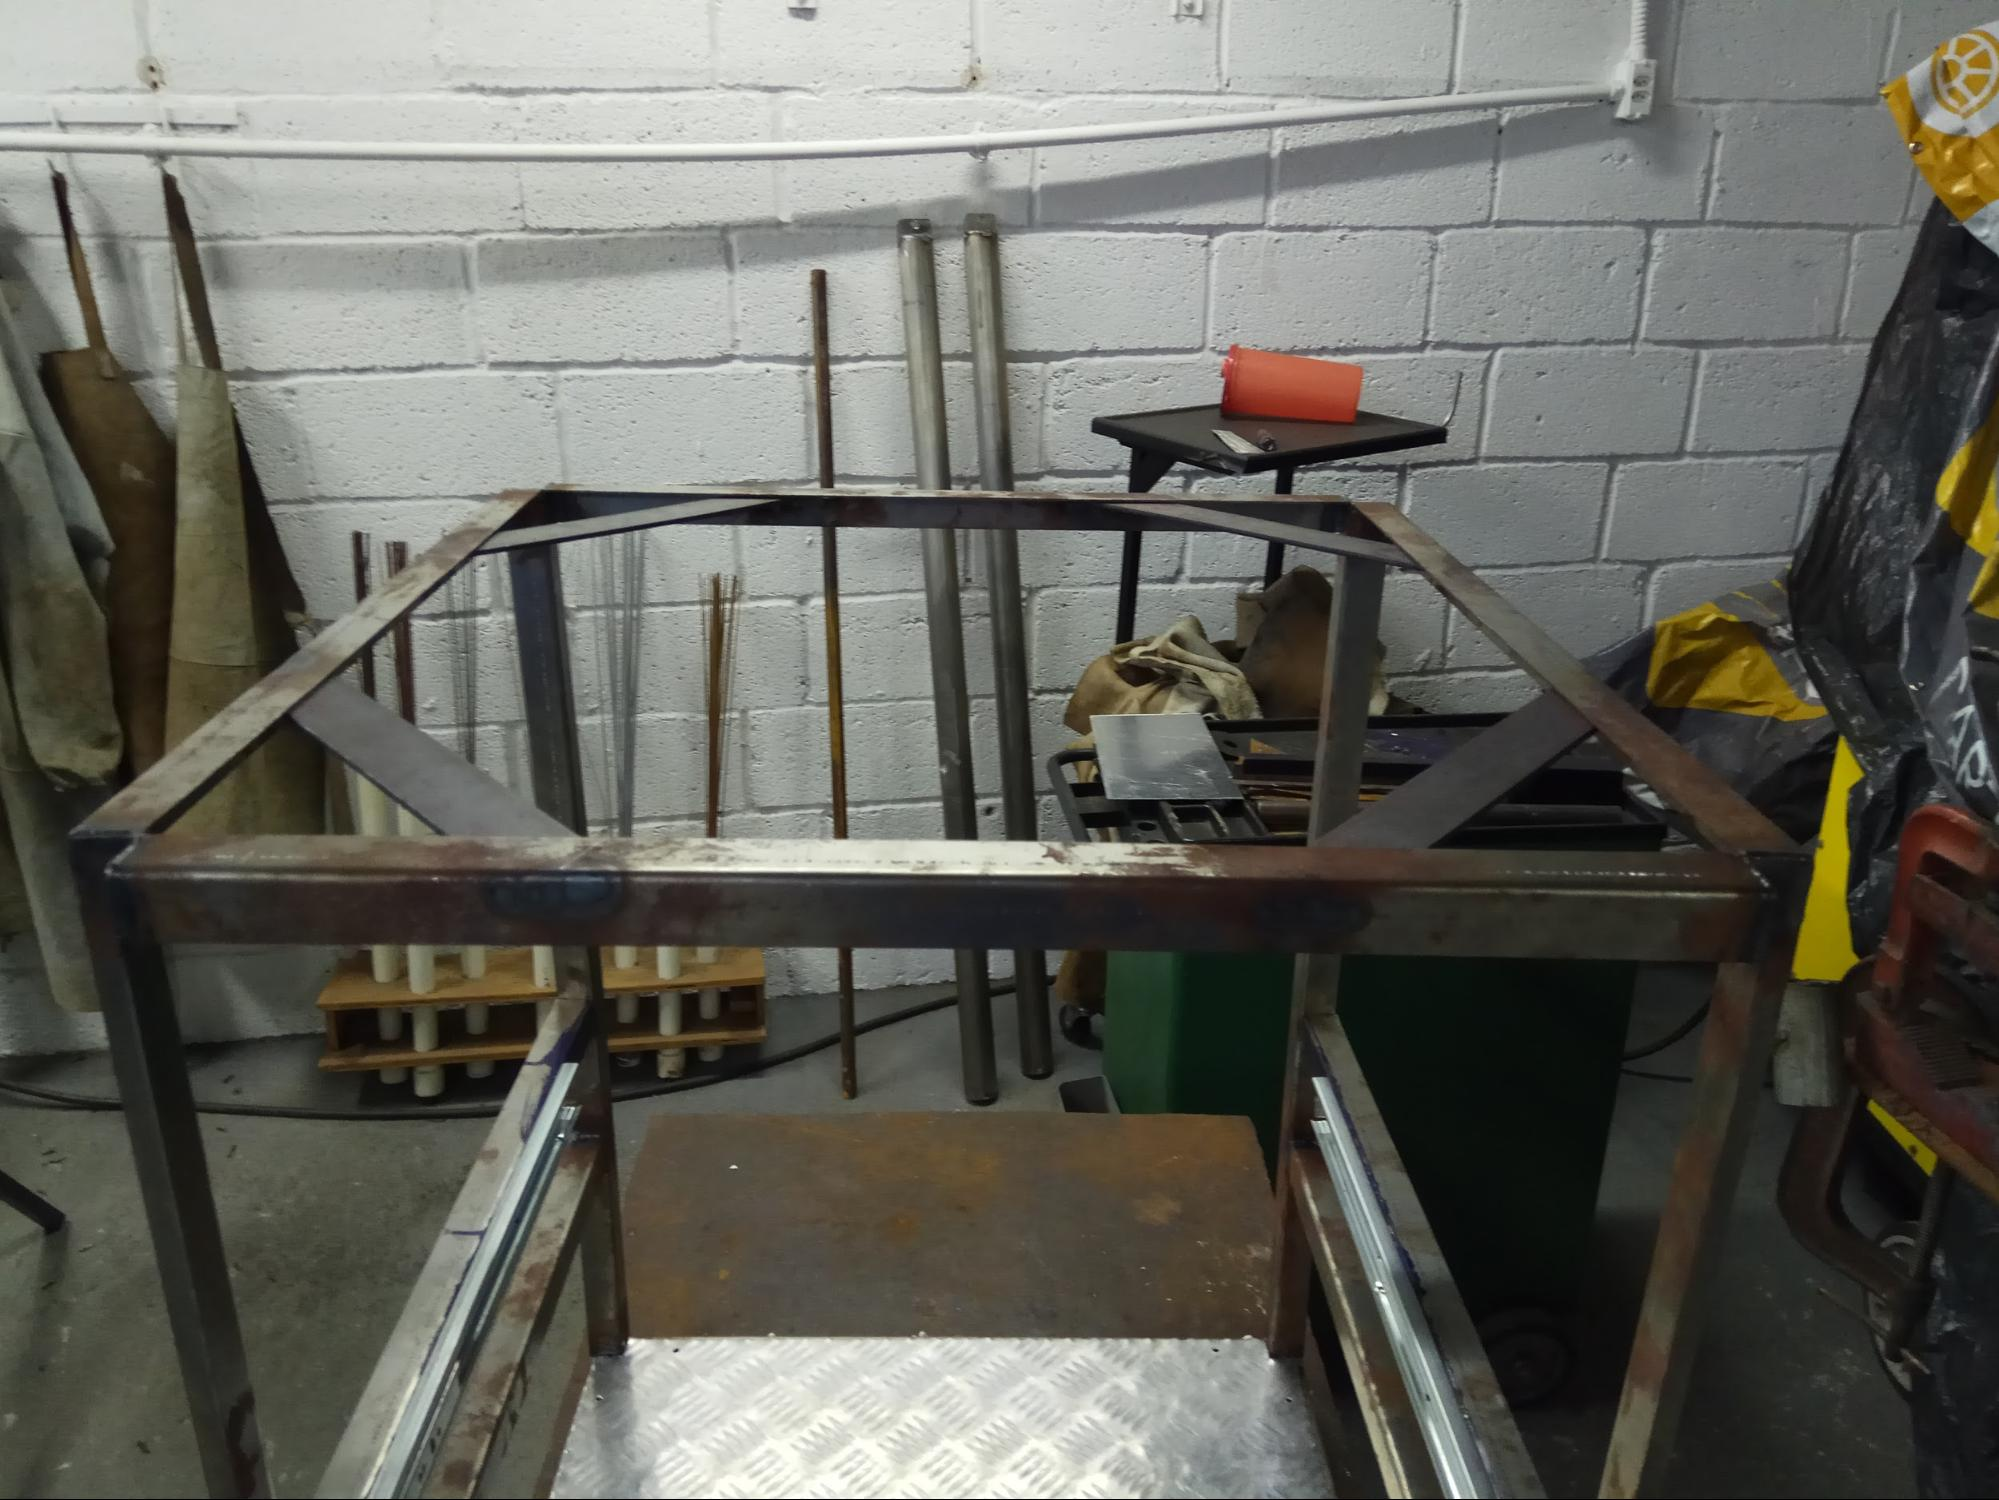
\includegraphics[width=11cm]{figuras/resultado_1.jpg}
	\caption{Parte superior da estrutura interna.} \label{resultado_1}
\end{figure}

\begin{figure}[H]
	\centering
	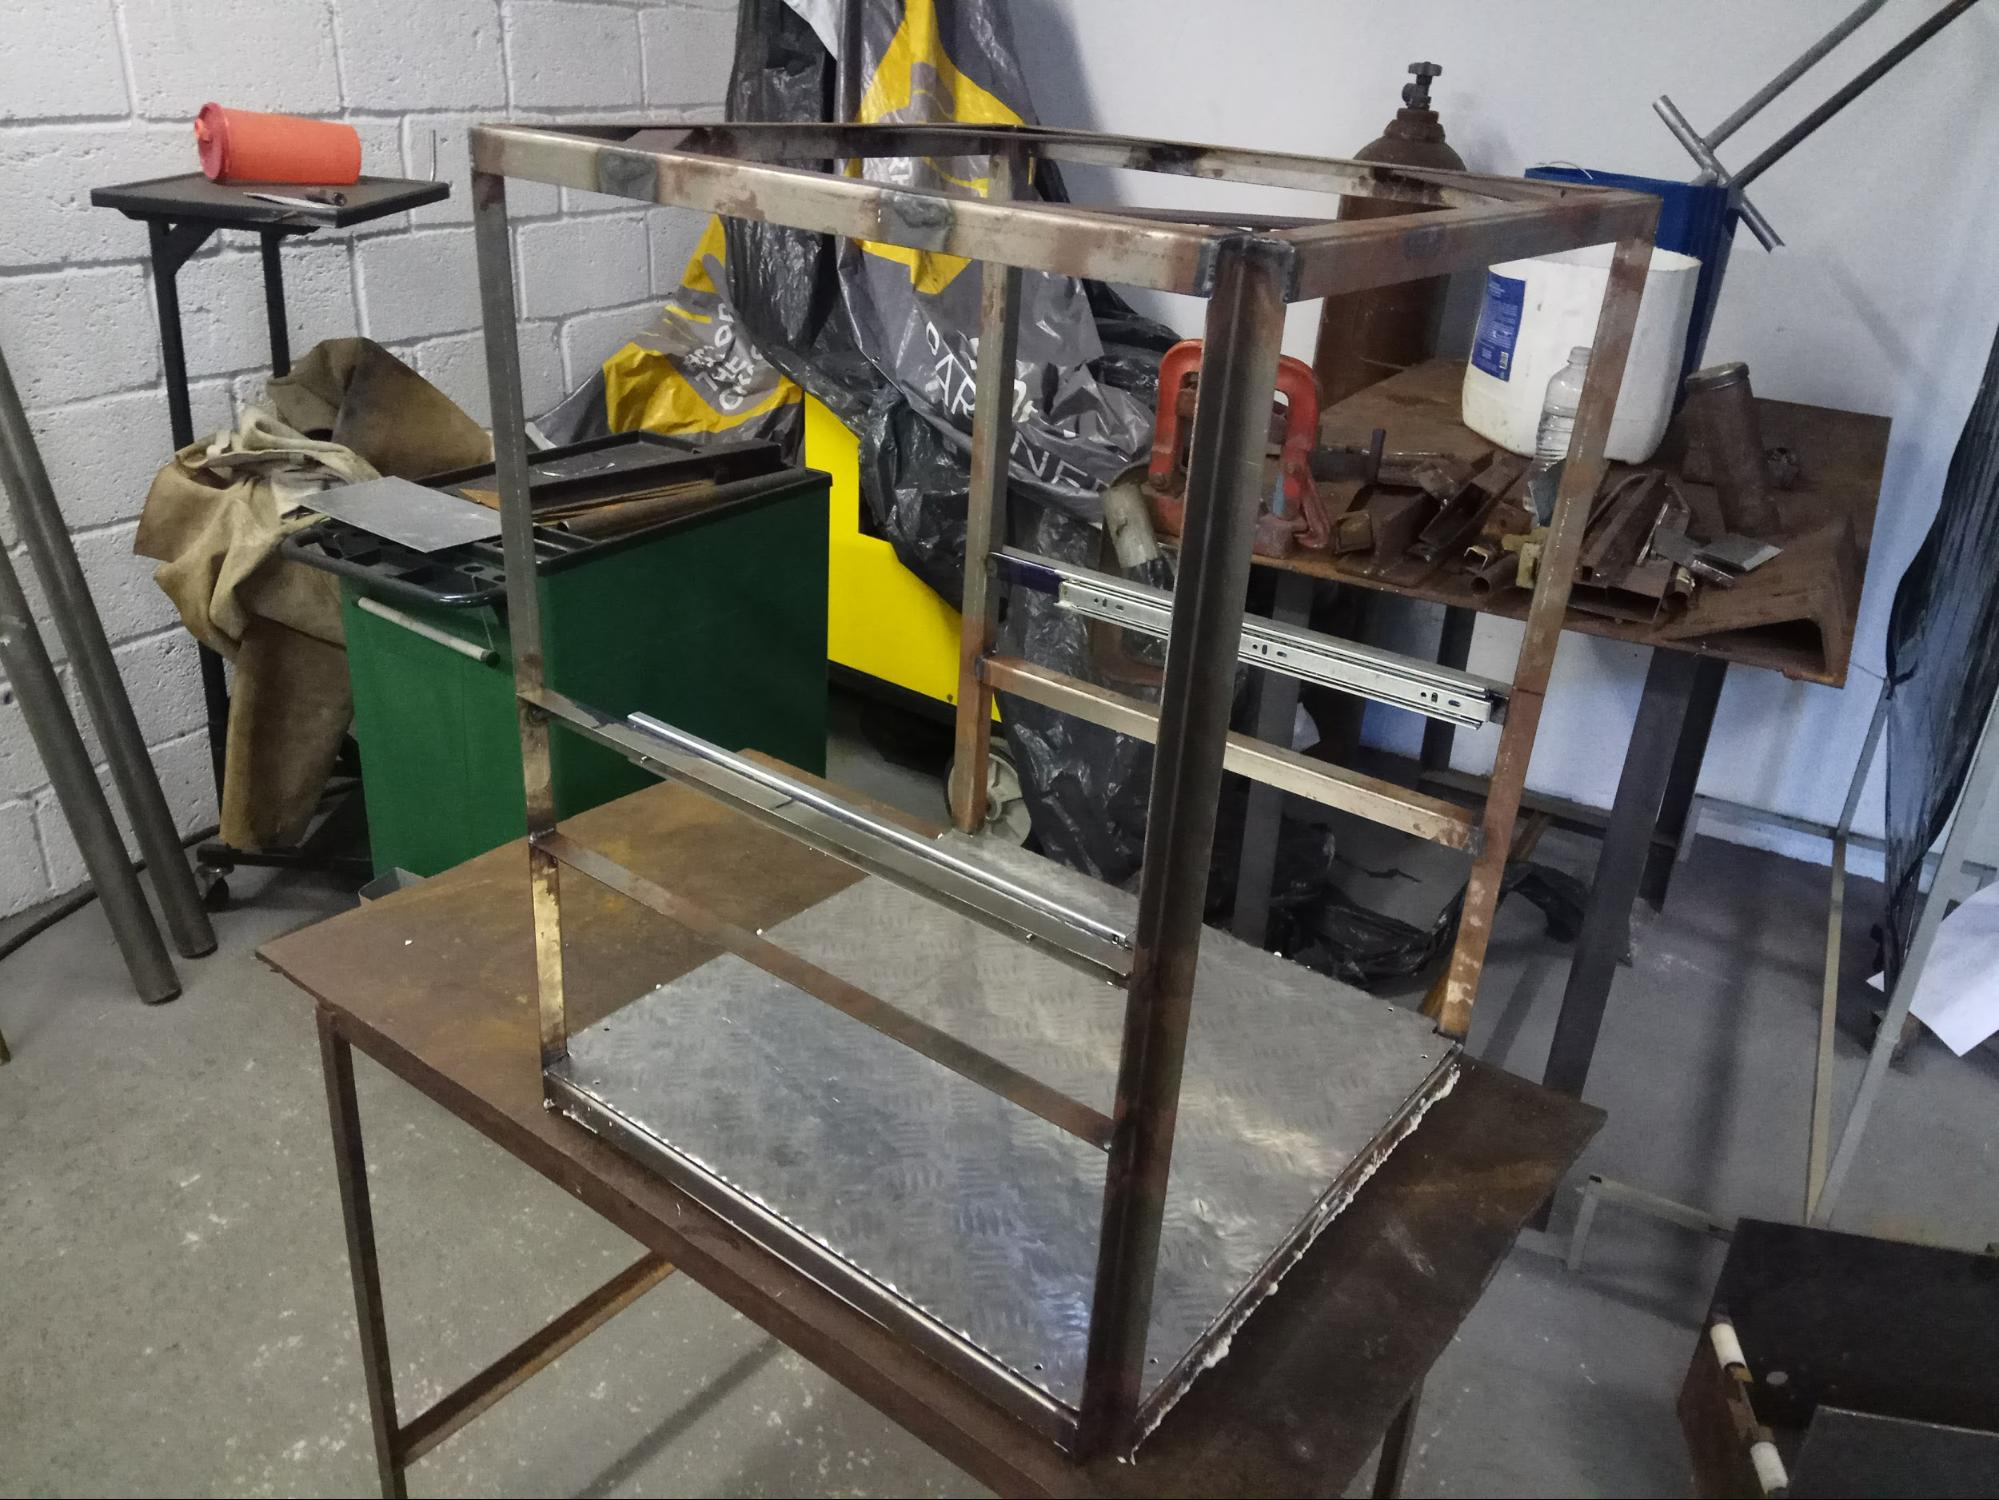
\includegraphics[width=11cm]{figuras/resultado_2.jpg}
	\caption{Corrediça telescópica onde comportará a gaveta de mudas.} \label{resultado_2}
\end{figure}

\section{Estrutura externa}

Materiais:
\begin{itemize}
	\item MDF
	\item Isopor
	\item PVC
	\item Silicone
	\item Espuma Expansiva
\end{itemize}

Fabricação:
\begin{itemize}
	\item	Foram realizadas medições da estrutura do Chassi, onde serão colocadas chapas de MDF para cobrir a estrutura, deixando a estrutura mais resistente, com um aspecto visual mais requintado. Na parte superior da estrutura, decidiu-se colocar MDF para fixar as lâmpadas, visto que anteriormente utilizaria-se isopor porém por questão de segurança decidiu-se fazer esta alteração.
	\item	Antes das chapas de MDF, foram alocadas placas de isopor como revestimento interno, onde foram cortados os espaços e instalaram-se alguns componentes como os Coolers nas laterais da estufa
	\item	Na parte interna, foram cortados placas de PVC de tamanho adequado, para compor a parte interna da estufa.
	\item	Serão utilizados silicone e espuma expansiva para realizar a junção das partes e para realizar o isolamento térmico da parte interna da estrutura.
\end{itemize}

A figura 46 mostram como ficou a parte externa até agora produzida.

\begin{figure}[H]
	\centering
	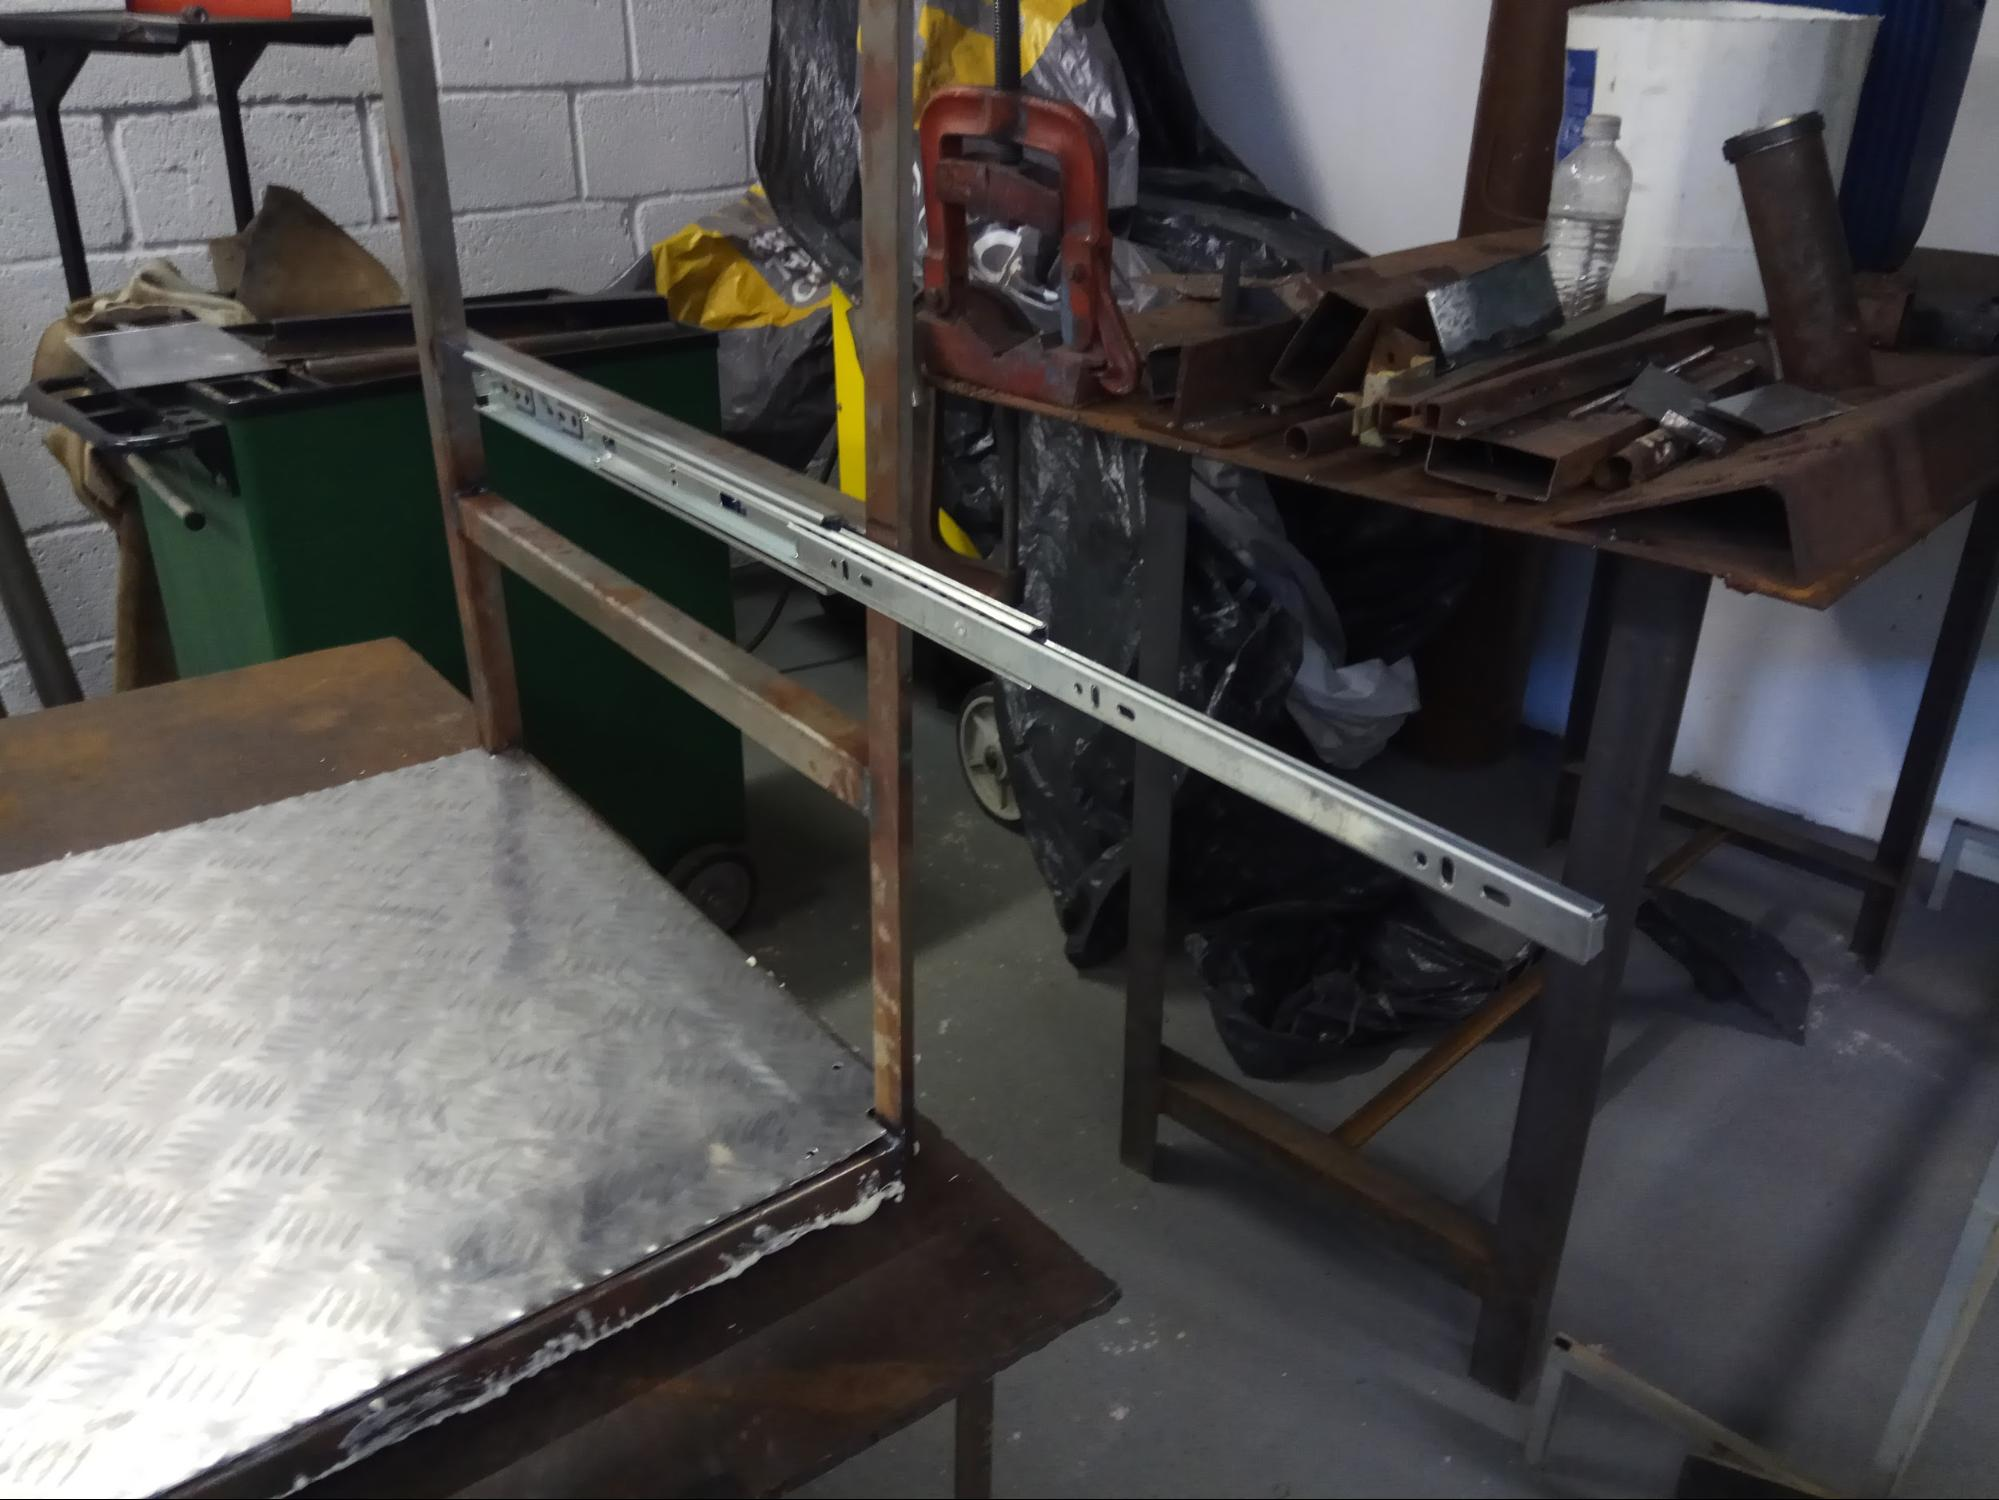
\includegraphics[width=12cm]{figuras/resultado_3.jpg}
	\caption{Estrutura com o isolamento externo.} \label{resultado_3}
\end{figure}